\section{Experimental results}
\label{sec:exp}

The experiments follow a mission similar to the original plan given in
Fig. \ref{fig:ex:plan}. The AUV needs to {\em Sample Vent2} and return
to the {\em surface} by the end of the mission. The AUV must also be
at the {\em surface} around
13:00. % with plans being produced by the europa planning engine
% \cite{frank2003}.
Fig. \ref{fig:ex:mixed1} demonstrates the resulting plan using
Algorithm \ref{alg:dispatch} using our executive \rx which synthesizes
temporal plans.

\begin{figure}[!htbp]
  \centering
  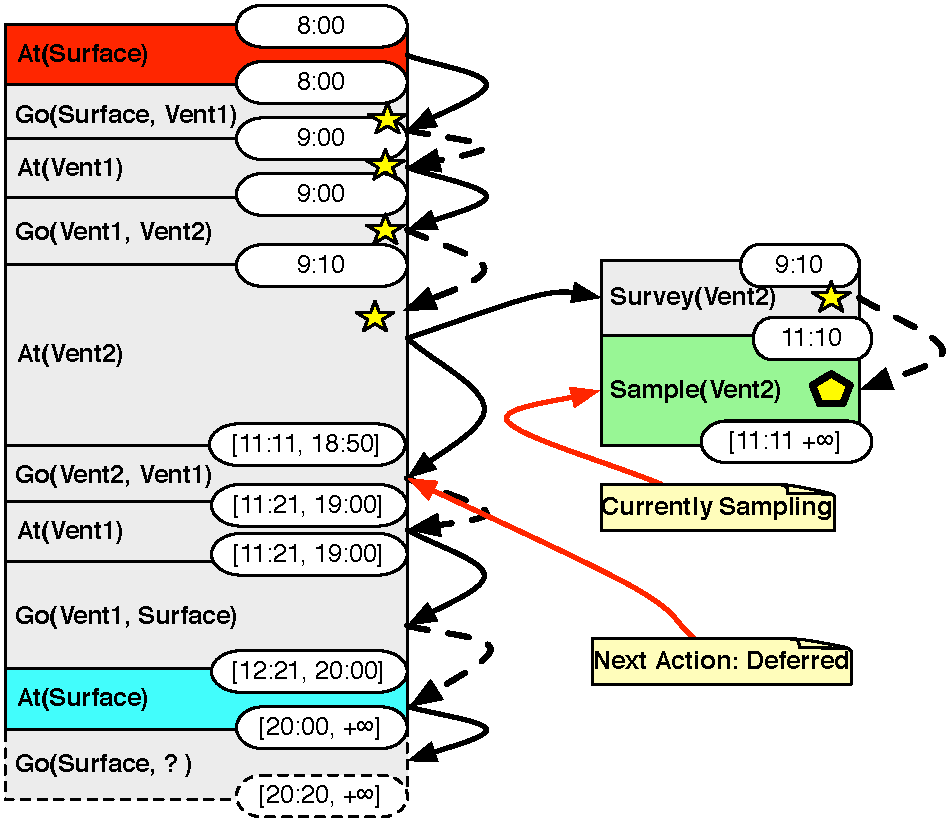
\includegraphics[width=0.8\columnwidth]{figs/example_MixedInitial}
  \caption{\small Plan solution from Fig. \ref{fig:ex:plan}. Solid
    lines indicate conditions and dashed lines indicate
    effects. Pentagons indicate {\em urgent} goals, stars indicate
    tokens that were deduced as {\em proactive}.}
  \label{fig:ex:mixed1}
\end{figure}

% For Algorithm \ref{SearchForGoal}, the search is straight forward. For
% example in 
From Fig. \ref{fig:ex:mixed1}, if the AUV is {\em At Surface} then the
next {\em Go} token will be dispatched. Because the search will follow
the causal links forward, where upon, it will find the goal {\em
  Sample Vent2} resulting in dispatching proactively.  Similarly, this
occurs for all of the tokens that are starred. The next token that is
not starred, {\em Go(Surface)}, is continuously searched but deferred,
because it is not connected to an urgent goal. The resulting AUV stays
at {\em Vent2} rather than heading to the {\em Surface} immediately.

%For the distributed algorithm approach, each token is checked during
%the creation of the plan to see if it is an external goal in
%$\Phi_{ge}$, or connected to one through a causal link. When the {\em
%Sample Vent2} is checked, we immediately find that it is a goal. We then
%follow the reverse causal link and find {\em Survey Vent2}.  However to
%better illustrate the algorithm, we can imagine that only the {\em Survey
%Vent2} has been causally connected to the goal so far. Therefore, we
%only star those two tokens. The path from {\em Surface} to {\em Vent1}
%to {\em Vent2} has yet to be built. When the path has finally been
%built, and {\em At Vent2} is checked, our algorithm searches one
%causal link and finds {\em Survey Vent2} which is starred. The search
%then follows the reverse causal link and stars the rest of the
%path. The starred tokens will then be proactively dispatched while the
%non-starred tokens will be deferred until later. Having similar
%results to Algorithm \ref{DispatchToken}.

In this run we then introduced a new {\em urgent} goal to {\em Sample
Vent1} at 11:30. We show the resulting plan in
Fig. \ref{fig:ex:mixed2}. There is not enough
time to {\em Sample Vent1} and be at the surface by 13:00. Therefore,
the goal is placed after the AUV goes to the surface. As a result the
actions which were so fdfar marked as deferred are now also causaly
linked to the new {\em urgent} goal. Therefore their former execution
policy is now updated. The resulting starred tokens in
Fig. \ref{fig:ex:mixed2} get dispatched proactively and includes all
the actions related to this mid-day surfacing goal.

\begin{figure}[t]
  \centering
  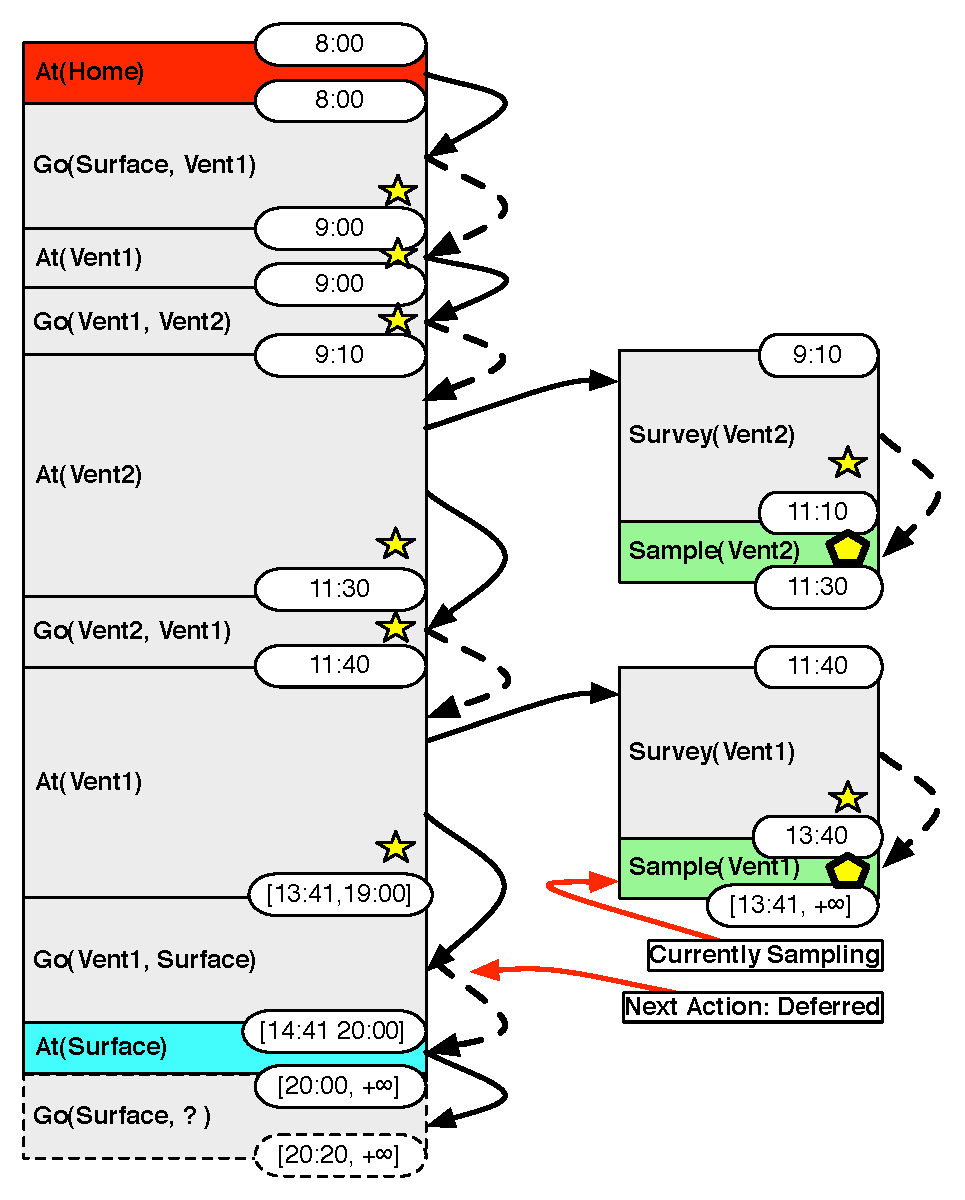
\includegraphics[width=0.8\columnwidth]{figs/example_MixedUpdate}
  \caption{\small The solution after receiving external request for
    the plan from Fig. \ref{fig:ex:mixed1}}
  \label{fig:ex:mixed2}
\end{figure}

Meanwhile the actions related to the last surfacing goal remains {\em
  deferred} and won't be executed until 19:00 allowing the vehicle to
sample {\em Vent1} for a duration of 2:50 hours.  After returning to the {\em
  Surface}, our planner and domain inserted a  partially instantiated
action to {\em Go(Surface, ?)} (dashed in the figures). 
This is an artifact resulting from the plan model which specifies that 
an {\em At} token is necessarily followed by a {\em Go}.
However, our algorithm will not be dispatching this token as it is not
connected to an {\em urgent} goal and its upper bound 
start time ($+\infty$) will not be met within the scope of the
mission. 

Next results focus on the overall performances of our algorithm. In our
experiments, the simulated AUV missions ran in a Linux virtual
machine. The virtual machine was run on a MacBook Pro and was 
allocated one core from a $2.33$ GHz Intel Core $2$ Duo processor. 
Time was recorded using a thread clock for the most accurate time.
The length of the mission was roughly 200 seconds. This was meant to allow many
simulations to be completed quickly. There is, however, no difference in 
performance if the mission were longer as the same plan would be produced
just with different timepoints.
 
Figure \ref{fig:example_run} shows a simulated mission run that
is similar to the original example in Fig. \ref{fig:ex:plan}.
However, in order to increase the complexity of the plan a
total of eight intermediate locations were added between the {\em
  surface} and {\em vent 1}. All the evaluation fo our algorithm 
done during the mission took less then $1ms$. For the most part the
largest spikes in performance were due to the need to evaluate the
dispatch for execution of both an {\em At} and ist following {\em Go}
tokens resulting on two searches within the plan. 

\begin{figure}[b]
  \centering
  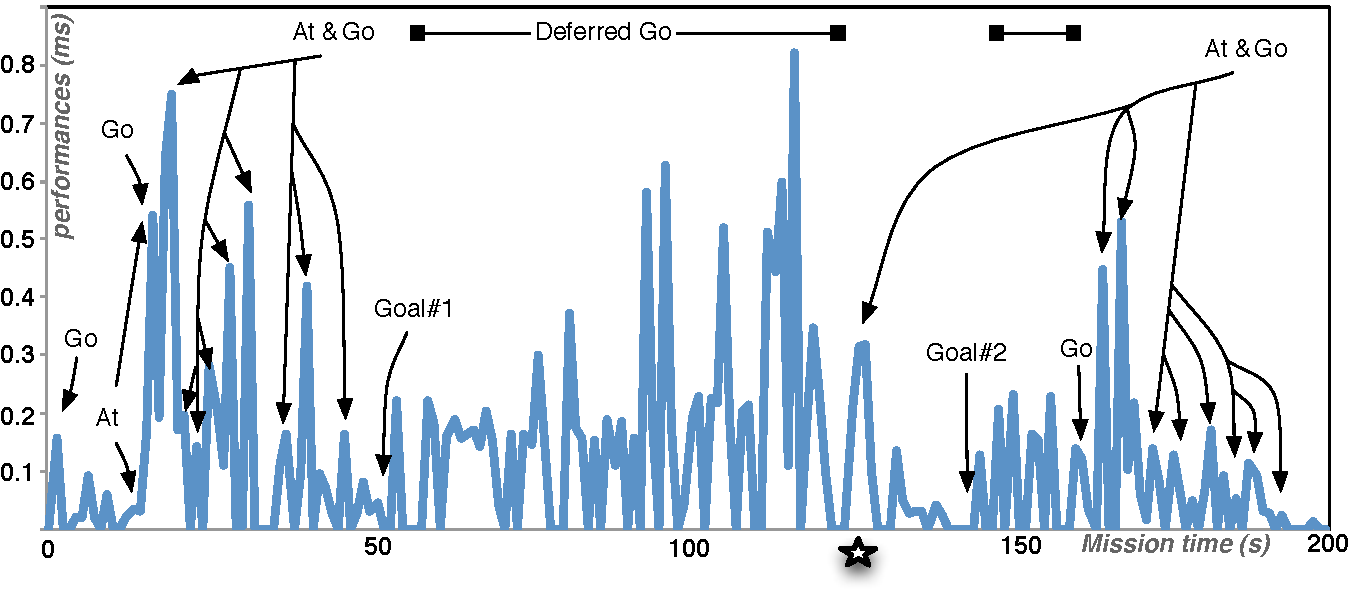
\includegraphics[width=\columnwidth]{figs/example_run.pdf}
  \caption{\small One mission run that shows the time needed for
    dispatching. The star represents when the Goal\#2 was received and
    integrated into the plan. Lines with boxes at the end represent
    the deferred action {\em Go} Because of space, we didn't put an
    arrow to every {\em At}. Our concern were the peaks that showed
    where the system had to dispatch both {\em At} and {\em Go}. }
  \label{fig:example_run}
\end{figure}

We also identifies a clear trend toward decreasing timing as 
the agent comes closer to either {\em Goal\#1} or {\em Goal\#2} 
completion. This is directly correlated to the reducing search
distance toward these goals as we execute new actions. 
We see however an important variability in execution time which is
most likely due to context switching between processes and threads 
within our agent as our virtual machine only had one processor. 
The bump in timing between the time-step $56$ and the introduction of
{\em Goal\#2} at time $127$ is due to the fact that our algorithm is
continuously searching the graph from the next {\em Go}, which during
this period, is not connected to an {\em urgent} goal. Due to the
resulting exhaustive search in the plan graph our algorithm execution
time during this period is on an average above $.2$
milliseconds. At tick $127$, the {\em Go} is no longer deferred and gets
dispatched quickly. The search for {\em Goal\#2} becomes relatively simple as it is
not very far away in the plan, and thus the time decreases
significantly.

\begin{figure}[!htbp]
  \centering
  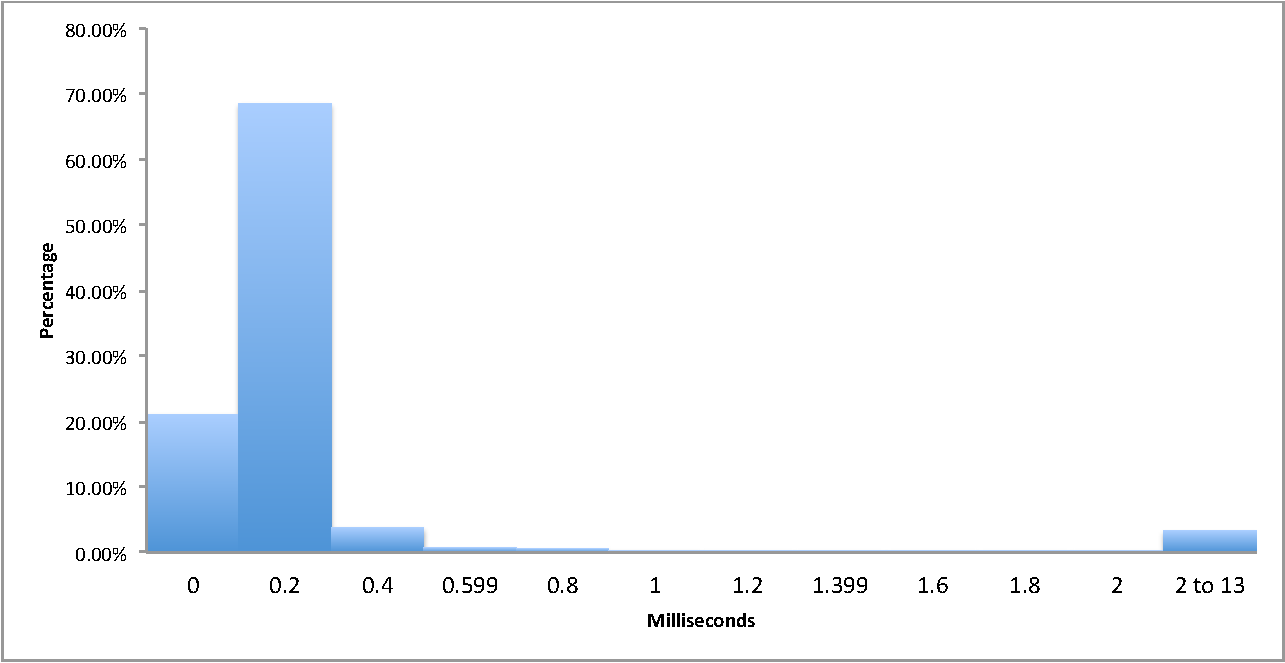
\includegraphics[width=\columnwidth]{figs/HistogramAlg1}
  \caption{\small Algorithm \ref{DispatchToken} was 
  timed at every increment of the mission time for $500$ 
  simulated missions. One goal was inserted into the plan 
  at a random time during the mission. The histogram shows 
  the distribution of the time, which is heavily skewed to the left.}
  \label{fig:histogram}
\end{figure}

In order to demonstrate the average amount of time that Algorithm
\ref{DispatchToken} uses, $500$ simulated missions were recorded and timed
at every increment of the mission time. Figure \ref{fig:histogram}
shows the distribution of execution time for all of these runs. We see
clearly that $90\%$ of the time our algorithm completed its serach in
in less than $0.2 ms$. The distribution is then long tailed with worst
performances between $2$ and $13ms$ occuring ofr less than $5\%$ of our
algorithm runs. Still these relatively pooor performances often did occur
when the {\em tokens} evaluated were meant to be {\em deferred} which
makes the small loss of performances not as critical.

%%% Local Variables: 
%%% mode: latex
%%% TeX-master: "aaai13"
%%% End: 
